\documentclass[a4paper,11pt]{report}

\author{A.~Umbach}
\title{Mein Maturaarbeitsthema}

\usepackage[ngerman]{babel}
\usepackage[latin1]{inputenc}
\usepackage{blindtext}
\usepackage{graphicx}

%minimale page header & footer
\usepackage{fancyhdr}
\pagestyle{fancy}
\setlength{\headheight}{14pt} 
\fancyhf{}
\fancyhead[C]{\nouppercase{\leftmark}}
\fancyfoot[C]{\thepage}

%create links in the pdf
\usepackage[colorlinks]{hyperref}

%a glossary
\usepackage[toc]{glossaries}


\newglossaryentry{glossar}
{
  name=Glossar,
  description={Im Glossar werden Fachausdr�cke und Abk�rzungen erkl�rt}
}
\newglossaryentry{blahblah}
{
  name=blahblah,
  description={\blindtext}
}

\makeglossary

\begin{document}
\maketitle
\tableofcontents

\chapter{Vorwort}
Hier kommt das Vorwort
\section{Warum \LaTeX{}}
Der Hauptgrund \LaTeX{} zu verwenden ist, damit man sich auf den Inhalt der Arbeit konzentrieren kann. Wie das ganze am Schluss aussehen soll, �berl�sst man dem Programm. Je weniger eigene konkrete Vorstellungen vom Layout man mitbringt, desto einfacher wird es.
\chapter{Einleitung}
In dieser Arbeit geht es um P

\chapter{Voraussetzungen}
\section{Vorwissen}
Um mit \LaTeX{} zu arbeiten, ist wenig Vorwissen notwendig. Allerdings sollte die Bereitschaft vorhanden sein, auch mal einen Blick ins Handbuch zu werfen, und wenn das nicht weiterhilft, Google nach der L�sung zu fragen.

\section{Ein wenig Text}
\blindtext

\chapter{Grundlagen}
\section{Kapitel und Unterkapitel}
\label{kapitelunterkapitel}
Mit \textbackslash chapter und \textbackslash section, bzw. \textbackslash subsection und \textbackslash subsubsection erstellt man Kapitel.

Abschnitte werden erzeugt, indem man einfach eine leere Zeile einf�gt. Um
Zeilenumbr�che muss man sich nicht k�mmern, diese entstehen automatisch.

\section{Abbildung}
Eine Abbildung ist auch mit ein paar Zeilen eingef�gt. Die Abbildungen werden auch automatisch nummeriert. Lena's Bild ist Abbildung \ref{lena}.
\begin{figure}
\begin{center}
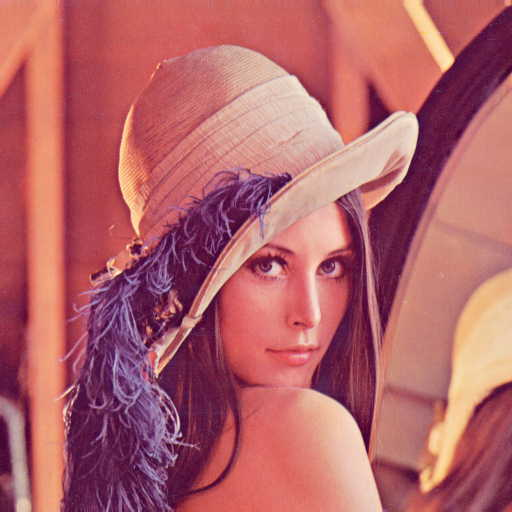
\includegraphics[width=0.6\textwidth]{lena.jpg}
\caption{Lena ist eins der Standardbilder aus der Bildverarbeitung}
\label{lena}
\end{center}
\end{figure}

\blindtext
\section{Verweise}
Mit \textbackslash ref und \textbackslash pageref k�nnen Verweise auf andere Kapitel bzw. Seiten erstellt werden. \emph{Kapitel und Unterkapitel} ist Kapitel \ref{kapitelunterkapitel} auf Seite \pageref{kapitelunterkapitel}.

\blindtext[2]

\section{Literaturverzeichnis}
Wie Tobias Oetiker \cite{lshort} schreibt, verwendet man \textbackslash cite um Literaturverweise und \textbackslash bibitem um das Literaturverzeichnis zu erstellen. Die \textbackslash bibitem Kommandos k�nnen dabei an einem beliebigen Ort, z.B. in einer separaten Datei oder am Ende des Dokuments stehen.

\begin{thebibliography}{99}
\bibitem{lshort} T. Oetiker:
\emph{The not so short introduction to \LaTeX{}}, Version 5.01, 2011
\end{thebibliography}



\chapter{F�r Fortgeschrittene}
\section{Das Glossar}
Im \gls{glossar} werden Fachausdr�cke und Abk�rzungen erkl�rt. Und hier noch ein weiterer Glossar-Eintrag: \gls{blahblah}

Gemeinerweise kann \LaTeX{} das Glossar nicht ganz alleine erstellen, es ist auf das externe Programm \emph{makeindex} angewiesen, um einen Index zu erzeugen. Dieses wird �ber die Kommanozeile aufgerufen. F�r diese Arbeit habe ich den Index mit
\\ \\
makeindex -s Maturaarbeit.ist -t Maturaarbeit.glg -o Maturaarbeit.gls Maturaarbeit.glo
\\ \\
erzeugt und anschliessend \LaTeX{} noch zweimal laufen lassen.

\printglossary[nonumberlist,title=Glossar]


\end{document}